\section{Methods}


\subsection{Data set}
Images from the ImageCLEF2012 Plant Identification Task were used in this study~\cite{imageclef2012}.
The data set consists of high resolution colour images that are labelled with metadata such as the full taxon name of the plant, its common name, and the GPS coordinates of the observation.
The images vary in resolution and aspect ratio but are scaled so that their longest axis is 800 pixels.
The data set originally contains three types of images: \emph{scans}, scan-like photographs (\emph{pseudoscans}), and normal \emph{photographs}.
Examples of these three types are shown in Figure~\vref{fig:imagetypes}.
They differ in the complexity of their backgrounds: \emph{scans} have a purely white background and few shadows, whereas \emph{pseudoscans}, while maintaining a uniform background, are more variable in the colour of their background and the lighting conditions.
Finally, \emph{photographs} have very diverse backgrounds, often with other plants visible, and vary strongly in their lighting conditions.


\begin{figure}[htb]
\centering
\resizebox{\textwidth}{!}{
\begin{tabular}{c@{\hskip 0.1in}c|c@{\hskip 0.1in}c|c@{\hskip 0.1in}c}
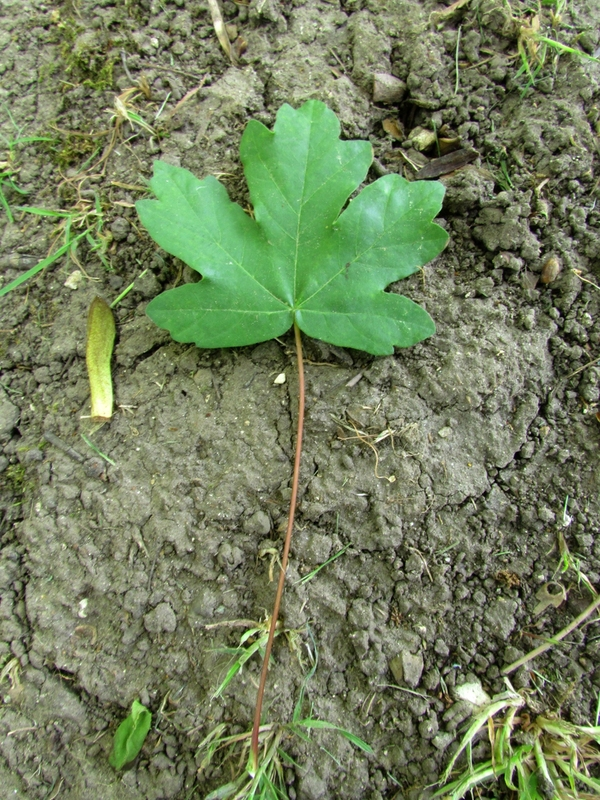
\includegraphics[width = .12\textwidth]{image/10733photograph.jpg} &
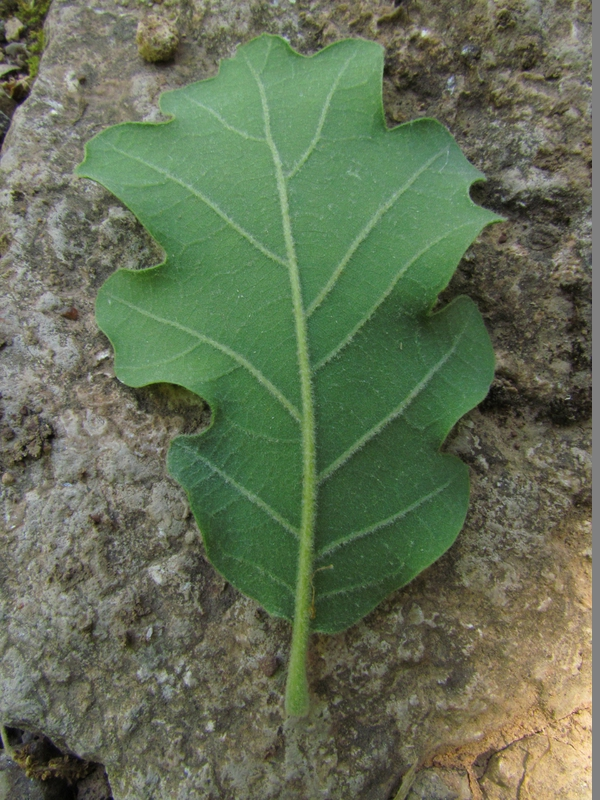
\includegraphics[width = .12\textwidth]{image/3702photograph.jpg} &
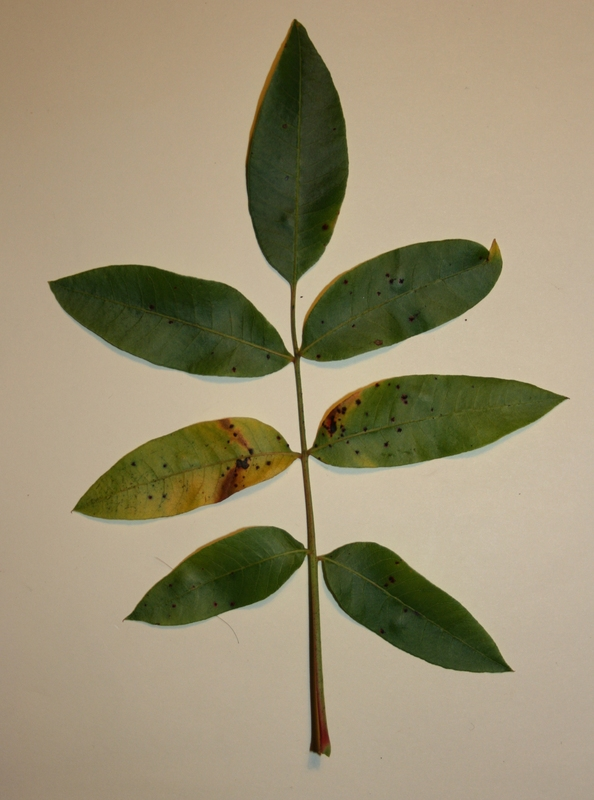
\includegraphics[width = .12\textwidth]{image/10513pseudoscan.jpg} &
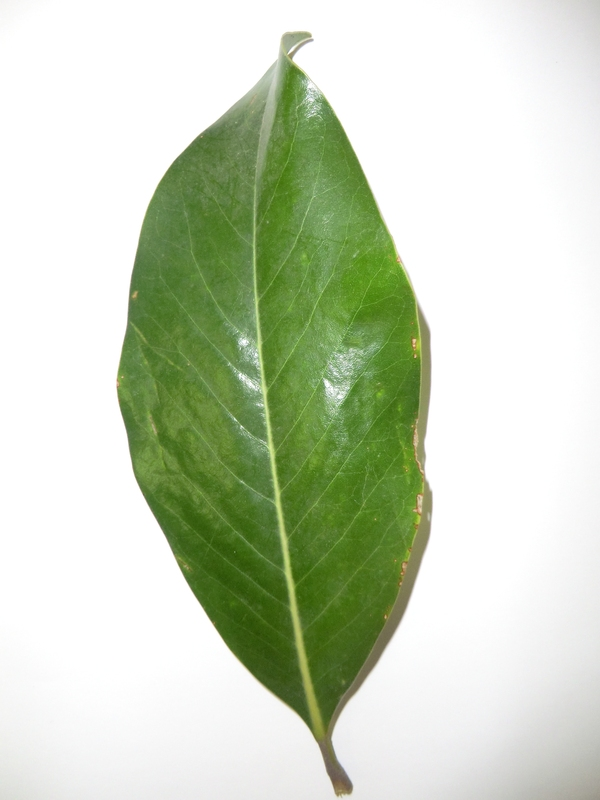
\includegraphics[width = .12\textwidth]{image/10145pseudoscan.jpg} &
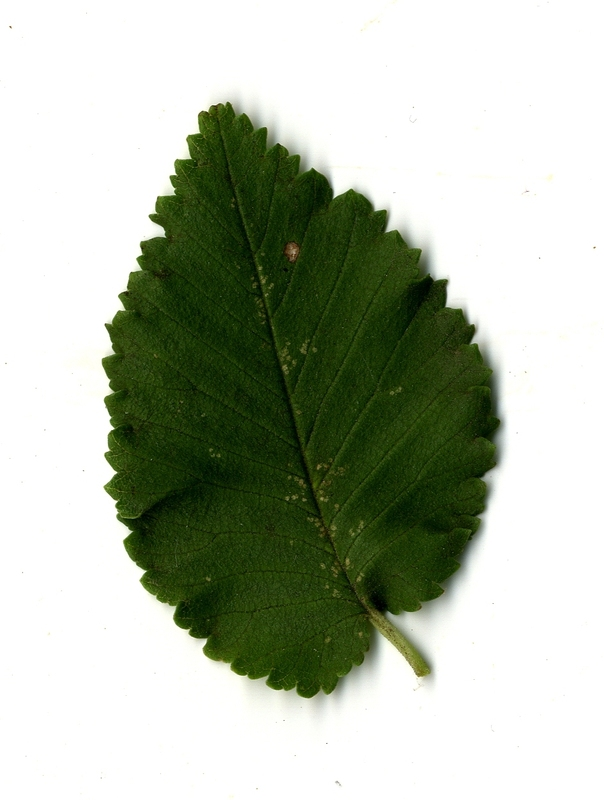
\includegraphics[width = .12\textwidth]{image/4564scan.jpg} &
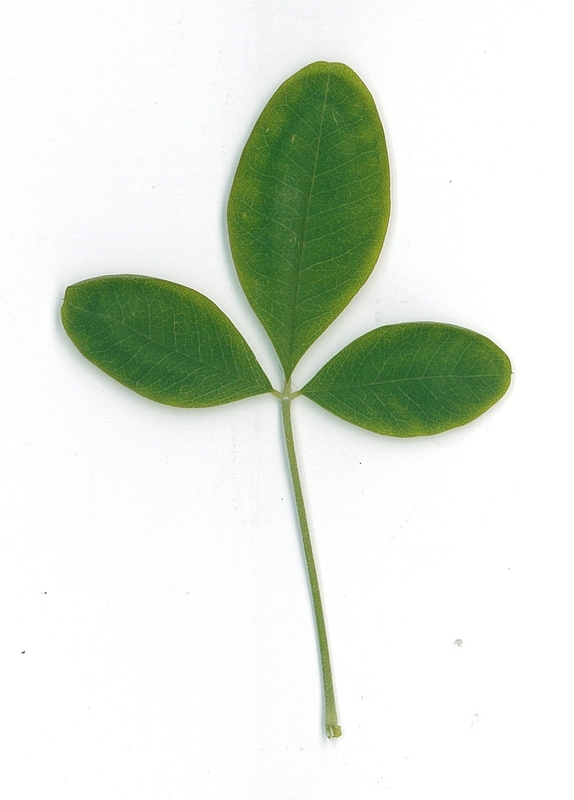
\includegraphics[width = .12\textwidth]{image/725scan.jpg}\\
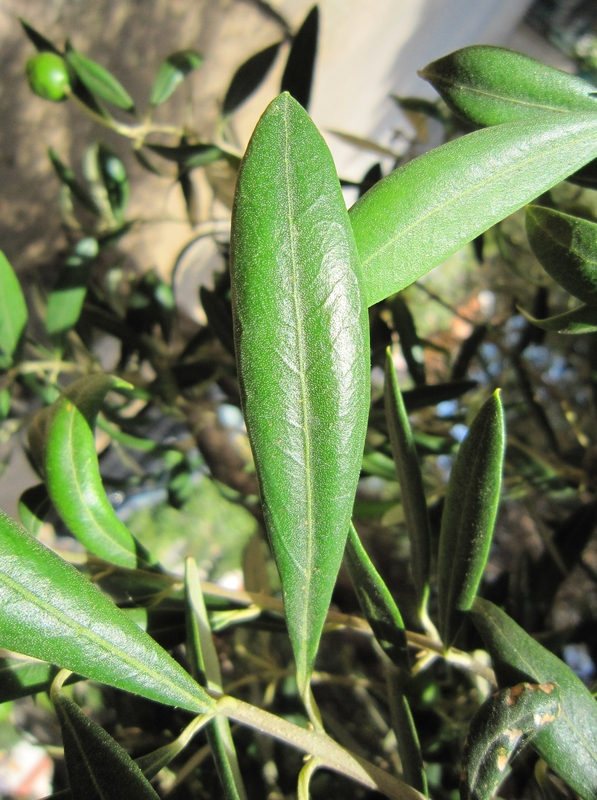
\includegraphics[width = .12\textwidth]{image/3589photograph.jpg} &
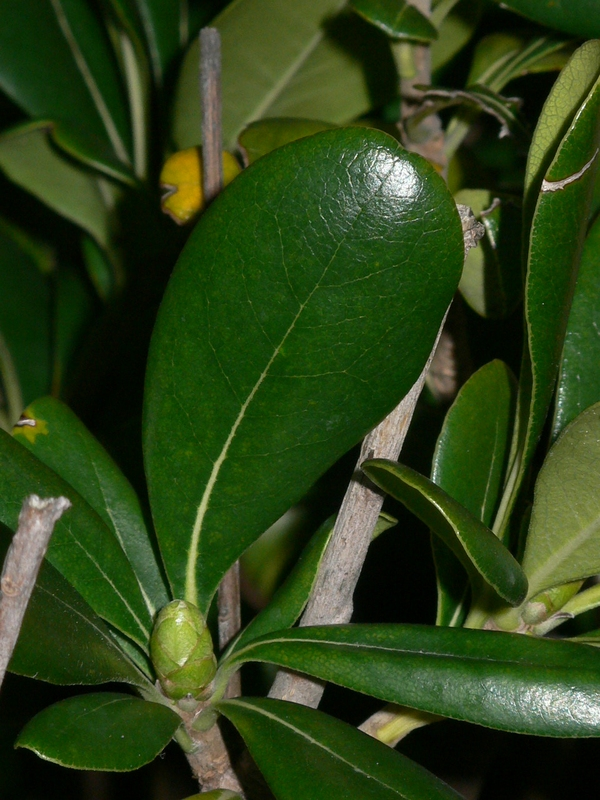
\includegraphics[width = .12\textwidth]{image/4717photograph.jpg} &
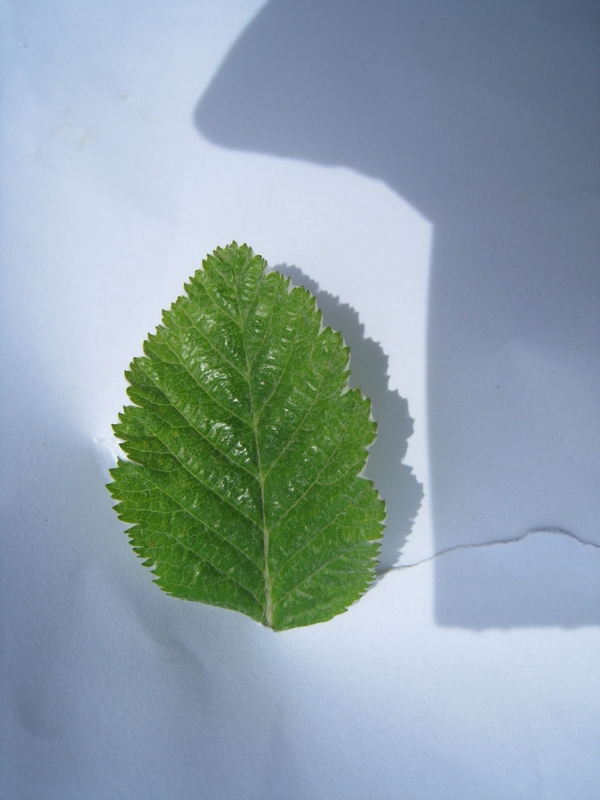
\includegraphics[width = .12\textwidth]{image/5093pseudoscan.jpg} &
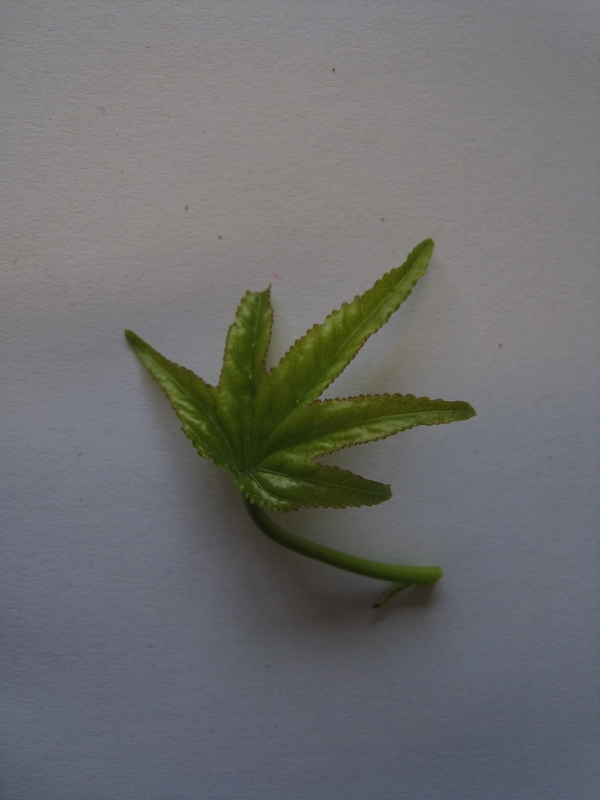
\includegraphics[width = .12\textwidth]{image/2655pseudoscan.jpg} &
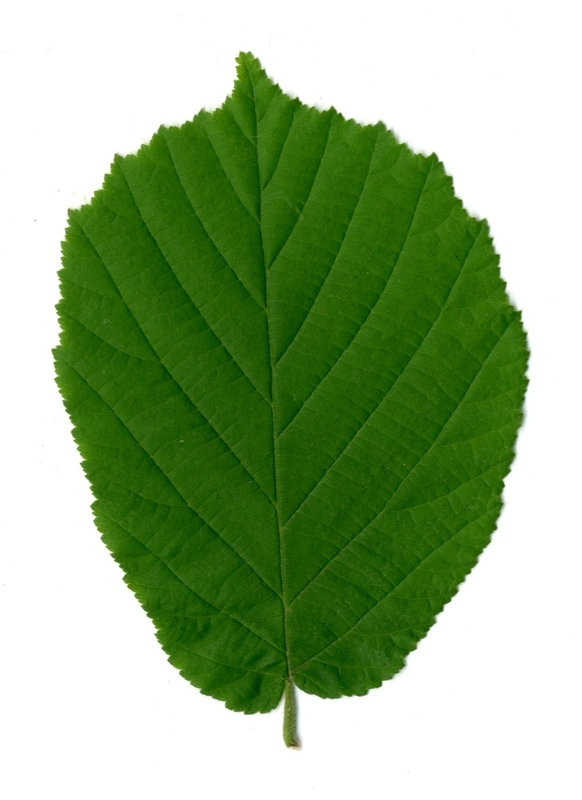
\includegraphics[width = .12\textwidth]{image/8736scan.jpg} &
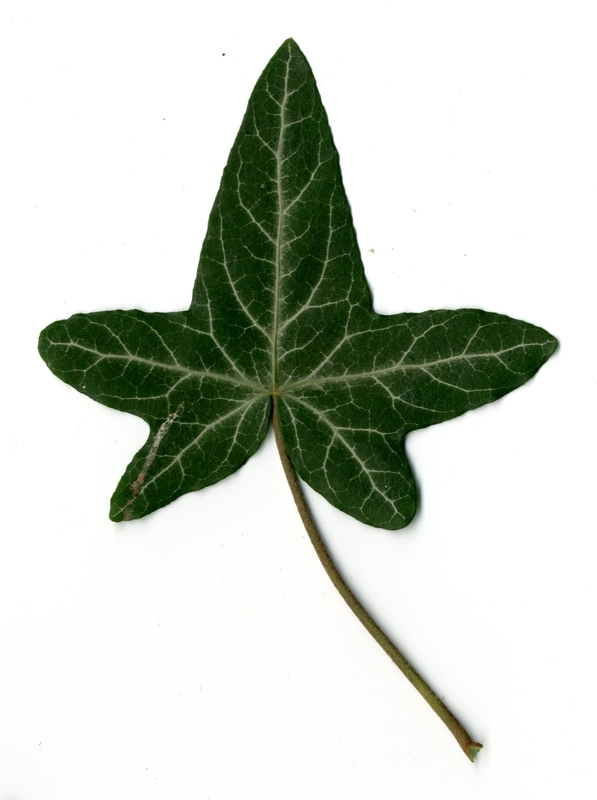
\includegraphics[width = .12\textwidth]{image/5292scan.jpg}
\end{tabular}
}
\caption{Examples of the three image types in the original ImageCLEF2012 data set. From left to right: \emph{photograph}, \emph{pseudoscan}, and \emph{scan}.}
\label{fig:imagetypes}
\end{figure}

Because of the complexity associated with extracting the leaf from its background, only \emph{scan} images (57\% of all images) were used in this study.
This subset consists of 6630 images of leaves from 75 classes.
The number of images varies strongly per class, from a single image (\emph{Xanthium strumarium}), to 367 (\emph{Ulmus minor}).
To resolve this imbalance only images from the 32 most frequent classes were used in this study. The least frequent of these 32 classes (\emph{Punica granatum}) still had 134 images.

%The images were divided into a training set of 4870 images ($\pm 73\%$) and a test set of 1760 images ($\pm 27\%$).
These images were divided into a training set of 2550 images ($\pm 73\%$) and a test set of 965 images ($\pm 27\%$).


\subsection{Feature extraction}
Several image classification studies~\cite{Wang2015, Lowe1999}, including at least one study into leaf image classification~\cite{Wang2011}, have made use of Scale-Invariant Feature Transform (SIFT) descriptors.
These descriptors are invariant to changes in scale and rotation, and somewhat robust to variations in viewpoint and illumination.
This makes them suitable for this task, since the leaves are photographed at varying scales and rotations.

% Images are converted to B/W, mask is applied.
% SIFT descriptors are extracted from area not covered by mask (the leaf).
% What does SIFT algorithm do, how does it work?
% Show keypoints in a nice image!
% ...

\subsection{Bag of visual words}
In spite of the SIFT descriptors' robustness to scale and rotation changes, it is unrealistic to expect features to be exactly identical between leaves, because of natural variation between leaves, and variation in the images that cannot be accounted for by SIFT.
Nevertheless we expect there to be certain natural features for each class that are recurrent in images of leaves of that class.
A good way to discover these features from the `noisy' SIFT descriptors is to use a clustering approach.
Each of the clusters that are found can then be considered to represent a certain feature that occurs multiple times in the data, albeit with some variation.

This study uses K-Means clustering with Euclidean distance as its distance metric~\cite{macqueen1967}.
A random subset of the total set of extracted SIFT descriptors is used for this process to mitigate the high computational cost caused by the high dimensionality of the SIFT descriptors (128 dimensions) and the large number of these descriptors.

Extracting clusters from the SIFT descriptors in this way allows for a much simpler description of the data.
Each cluster centre represents a \emph{visual word} (or code word).
Together the set of cluster centres forms a dictionary (or bag) of visual words.
Using this dictionary any image in the data set can be described in terms of its visual words.
This process starts by extracting the SIFT descriptors from the image.
These descriptors are then individually assigned to the existing clusters nearest to them using K-Nearest Neighbour.
This step translates the descriptors from ones that are specific to the image to more general descriptors that represent certain visual words.
Now that the image's features are expressed in terms of the visual words in the dictionary, a histogram can be made depicting the frequency of each visual word in the image.
This histogram has a fixed length $K$ --- the number of visual words in the dictionary.

A challenge of this approach is to find the optimal value of $K$.
If $K$ is too small, the vocabulary will be too limited to accurately describe all features, since the clusters that form will be too general.
Conversely, if $K$ is too large, too much of the original noise will still be present in the clusters, as there will be many small clusters that describe small variations of the same underlying feature. 
This defeats the purpose of the bag-of-words approach by not really describing the images in more general terms.

In this study $K$ was selected through a procedure in which classifier performance was compared for a range of values of $K$, between 50 and 250 (based on~\cite{Nguy2013}).



\subsection{Classifiers}

\subsubsection{Neural network}
For this research a neural network, with backward propagation of errors, was used as the main classifier for the extracted image data. As our optimization method we used gradient descent. The network consisted of an input layer, one hidden layer and an output layer.\\
As our classifier used supervised learning we needed to specify target output and compare it to the output given by the network. For the output we used $N_{output}$ output nodes where $N_{output}=N_{leaftypes}$. The target consisted of a vector $V=[..,0,0,0,..]$ of length $N_{leaftypes}$ where $V[I_{leaftype}]=1$. The index $I_{leaftype}$ was unique for every leaf type and corresponded to its index in the leaf type dictionary. The amount of input nodes was $N_{input}=Length_{histogram}$ The optimal amount of hidden nodes was $N_{hidden}=100$ and were randomly initialized from a continuous uniform distribution of the interval $[-1, 1]$.\\
As the activation function the sigmoid function was chosen, defined by $$f(x)=\frac{1}{1+e^{-x}}$$
Where its derivative is as follows:
$$f'(x)=f(x)(1-f(x))$$
A learning value of $0.01$ was used for all weights including those of the bias nodes of which there were 2, one connected to the hidden layer and one connected to the output layer. The option for regularization, that discourages large changes in weights, was also added, but later discarded as no improvements were shown for various values of the regularization lambda. Another change made was the removal of mini-batch learning in favour of online learning, although improving the time till convergence, it reduced accuracy and was therefore dropped from the network.\\
In order to avoid the program to learn meaning from the order of input data we presented the data in a randomized order every epoch. This counteracts repeating update cycles.

\subsubsection{KNN}
A K-Nearest Neighbour classifier was made to serve as a comparison for the neural network's performance.
The classifier finds the $K$ nearest neighbours of a test image's bag-of-words histogram (using Euclidean distance) and assigns it the majority class.
In case of a tie the class assignment is chosen randomly from the tied competitors.
The classifier returns a list of the top $T$ classes.
Following~\cite{Wang2011, Belh2008}, a classification is considered to be correct if the ground truth class appears in the top 5 results. 
